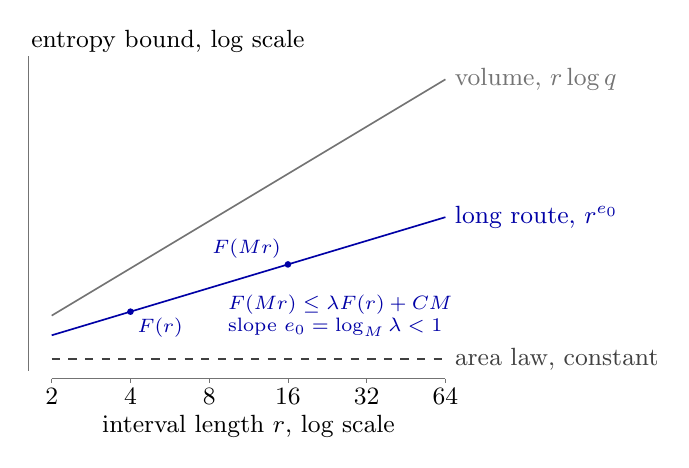
\begin{tikzpicture}[x=1cm, y=1cm, line width=0.3pt,
    lab/.style={font=\small, inner sep=1pt},
    name/.style={font=\scriptsize, text=black!55, inner sep=1pt},
    bound/.style={line width=0.6pt}]
  \def\dx{1.0}\def\dy{0.6}
  \def\xmax{5.0}\def\ymax{4.1}
  \draw[black!55] (0, 0) -- (\xmax, 0);
  \draw[black!55] (-0.3, 0.1) -- (-0.3, \ymax);
  \foreach \k/\r in {0/2, 1/4, 2/8, 3/16, 4/32, 5/64} {
    \draw[black!55] (\k*\dx, 0) -- (\k*\dx, -0.06);
    \node[lab, anchor=north] at (\k*\dx, -0.08) {\(\r\)};
  }
  \node[lab, anchor=north] at (2.5*\dx, -0.42) {interval length \(r\), log scale};
  \node[lab, anchor=south west] at (-0.3, \ymax) {entropy bound, log scale};
  \draw[bound, black!55] (0, 0.8) -- (5*\dx, {0.8 + 5*\dy});
  \node[lab, anchor=west, text=black!55] at (5*\dx + 0.08, {0.8 + 5*\dy}) {volume, \(r\log q\)};
  \draw[bound, blue!65!black] (0, 0.55) -- (5*\dx, {0.55 + 2.5*\dy});
  \node[lab, anchor=west, text=blue!65!black] at (5*\dx + 0.08, {0.55 + 2.5*\dy}) {long route, \(r^{e_0}\)};
  \draw[bound, dashed, black!75] (0, 0.25) -- (5*\dx, 0.25);
  \node[lab, anchor=west, text=black!75] at (5*\dx + 0.08, 0.25) {area law, constant};
  \fill[blue!65!black] (1*\dx, {0.55 + 0.5*\dy}) circle (1.2pt);
  \fill[blue!65!black] (3*\dx, {0.55 + 1.5*\dy}) circle (1.2pt);
  \node[name, anchor=north west, text=blue!65!black] at (1*\dx + 0.05, {0.55 + 0.5*\dy - 0.04}) {\(F(r)\)};
  \node[name, anchor=south east, text=blue!65!black] at (3*\dx - 0.05, {0.55 + 1.5*\dy + 0.04}) {\(F(Mr)\)};
  \node[name, anchor=north west, align=left, text=blue!65!black] at (2.2*\dx, 1.1)
    {\(F(Mr)\le\lambda F(r)+CM\)\\ slope \(e_0=\log_M\lambda<1\)};
\end{tikzpicture}
